% !TeX spellcheck = en_US
\documentclass[french]{yLectureNote}

\title{Électrocinétique}
\subtitle{Physique}
\author{Paulhenry Saux}
\date{\today}
\yLanguage{Français}

\professor{Allard}%allard@irsamc.ups-tlse.fr
\usepackage{graphicx}%----pour mettre des images
\usepackage[utf8]{inputenc}%---encodage
\usepackage{geometry}%---pour modifier les tailles et mettre a4paper
%\usepackage{awesomebox}%---pour les boites d'exercices, de pbq et de croquis ---d\'esactiv\'e pour les TP de PC
\usepackage{tikz}%---pour deiffner + d\'ependance de chemfig
\usepackage{tkz-tab}
\usepackage{chemfig}%---pour deiffner formules chimiques
\usepackage{chemformula}%---pour les formules chimiques en \'equation : \ch{...}
\usepackage{tabularx}%---pour dimensionner automatiquement les tableaux avec variable X
\usepackage{awesomebox}%---Pour les boites info, danger et autres
\usepackage{menukeys}%---Pour deiffner les touches de Calculatrice
\usepackage{fancyhdr}%---pour les en-t\^ete personnalis\'ees
\usepackage{blindtext}%---pour les liens
\usepackage{hyperref}%---pour les liens (\`a mettre en dernier)
\usepackage{caption}%---pour la francisation de la l\'egende table vers Tableau
\usepackage{pifont}
\usepackage{array}%---pour les tableaux
\usepackage{lipsum}
\usepackage{yFlatTable}
\usepackage{multicol}
\newcommand{\Lim}[1]{\lim\limits_{\substack{#1}}\:}
\renewcommand{\vec}{\overrightarrow}
\begin{document}

	\chapter{Introduction}
	%\section{Introduction}
\section{Charge et courant}
\subsection{Charge}
\subsubsection{Définition et valeurs}
\begin{definition}[Charge électrique]
Propriété fondamentale de la matière qui caractérise son intéraction avec les champs électromagnétiques
%Elle peut \^etre > 0 et < 0 et son unité est le Coulomb.
\end{definition}
Elle est quantifiée : c'est un multiple entier de la charge élémentaire \(e  = 1.602\cdot 10^{-19}\) C
\begin{itemize}
 \item électron : $q_{e-} = -e$
 \item proton : $q_{e} = +e$
 \item neutron : $q_n = 0$
\end{itemize}
% \subsubsection{Couplage entre particule}
% Le couplage entre une particule de masse $m$ et un champ EM s'écrit sous la forme d'une force appelée force de Lorenz, avec \(\vec{E}\) le champ électrique et \(\vec{B}\) le champ magnétique : \[\vec{F} = q(\vec{E} + \vec{v} \wedge \vec{B})\]
\subsection{Courant}
\subsubsection{Définition}
\begin{definition}[Courant]
C'est le débit de charge dans un conducteur, noté \(i(t) = \frac{\mathrm{d} q(t)}{\mathrm{d}t}\). Il peut \^etre continu (les charges se déplacent dans le m\^eme sens) ou alternatif (sens du déplacement oscille).
\end{definition}
Il est mesuré par l'intensité du courant et s'exprime en Ampère : $C/s$
% \subsubsection{ODG}
% \(1A \Rightarrow D = \frac{I}{e} = 6\cdot 10^{18} \)
\section{Potentiel électrique, tension et dip\^oles}
\subsection{Définitions}
% Pour faire se déplacer des charges, il faut qu'elles soient attirées par la force de Lorenz vers les potentiels plus faible.
%
% Le travail de la force électrique pour amener les charges de A à B sécrit comme \(W_{AB} = \int \vec{F}\cdot \vec{u}\), avec \(\vec{F} = - \vec{\nabla} E_p\).
\begin{definition}[Tension électrique]

On appelle tension électrique la différence de potentielle \(u_{AB} = V_A - V_B = \frac{Ep(A)-Ep(B)}{q}\). Elle traduit le changement de potentiel de la charge $q$ entre \(A\) et \(B\) et s'exprime en Volt.
\end{definition}
\begin{definition}[Dip\^ole]
Un composant qui possède deux p\^oles, appelées bornes. Ils fournissent ou consomment de l'énergie/puissance.
\end{definition}
\begin{definition}[Puissance]
Elle correspond au débit d'énergie à travers le dip\^ole et s'exprime en Watt (J/s). Dans un circuit la puissance fournie est intégralement consommée.
\end{definition}
\begin{definition}[Circuit]
Un ensemble de dip\^oles reliés par des fils électriques idéaux (conducteur parfait). Deux points reliés par un conduteur parfait sont au m\^eme potentiel
\end{definition}
\subsection{Conventions}
\subsubsection{Générateur}
La puissance le traversant est négative : \(P<0\) et le sens positif du courant est orienté comme la tension.
\subsubsection{Récepteur}
La puissance le traversant est positive : \(P>0\) et le sens positif du courant est orienté dans le sens {\color{criticalColor}opposé} à la tension.

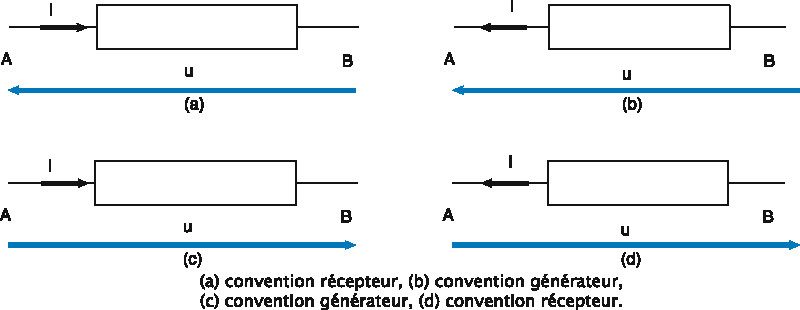
\includegraphics[scale=0.7]{fig-conventions}
\section{Dip\^oles élémentaires}
Ils permettent en les assemblant  de modéliser le comportement électrique de tout circuit électrique réel. Ils sont parcourus par un courant et ont une tension à leur borne. On caractérise leur propriété par une courbe courant/tension de la forme \(i = f(u)\). Cette courbe se nomme carractéristique courant/tension.
\subsection{Générateur de tension idéal}
Il impose une tension $U_0$ assez grande entre ses bornes quelque soit le dip\^ole auquel il est connecté.

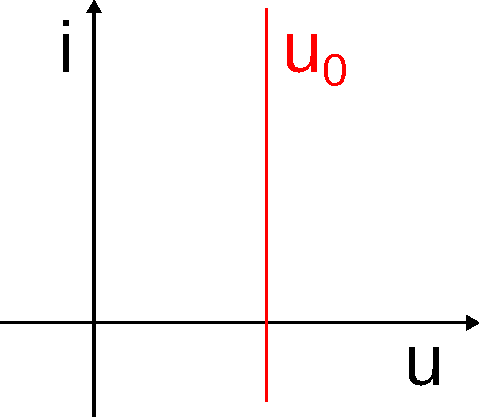
\includegraphics[scale=0.3]{c1-fig1}
\subsection{Générateur de courant idéal}
Il maintient un courant $I_0$ constant quelque soit les dip\^oles connectés 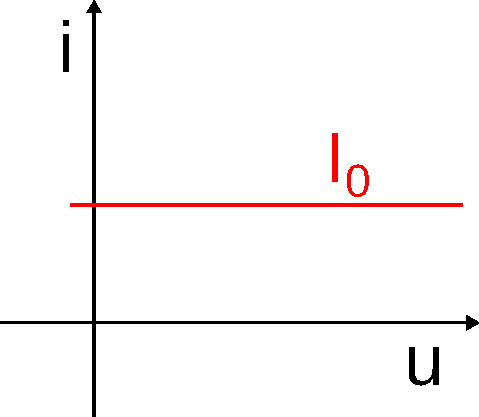
\includegraphics[scale=0.3]{c1-fig2}
\subsection{Résistance}
C'est un dip\^ole récepteur dont la tension entre ses bornes est proportionnelle au courant qui le traverse avec un coefficient de proportionalité $R$ en $\Omega$. On a $U=R\times I$. C'est le seul dip\^ole à dissiper l'énergie sous forme de chaleur par effet Joule

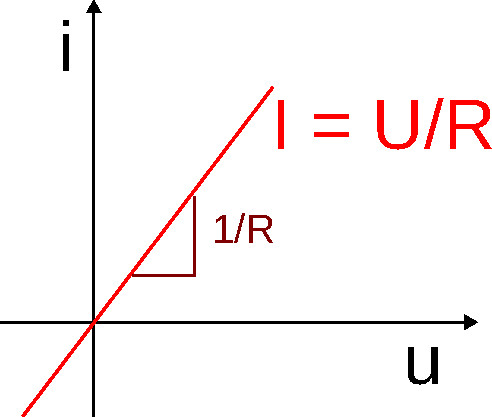
\includegraphics[scale=0.3]{c1-fig3}
\subsection{Condensateur idéal}
C'est un sip\^ole dont la tension à ses bornes et le courant sont reliés par $i = C \frac{\mathrm{d}U}{\mathrm{d}t}$ ou $U = \frac{q}{C}$ avec $q$ la charge accumulée dans le condensateur. et $C$ la capacité du condensateur qui s'exprime en Farad $F$.

Pour une tension constante, on a un courant nul, donc il se comporte comme un interrupteur couvert.

%On encerlce 2 plaques avec un solant au milieu

% La capcité dépend de la surface des plaques, de la distance entre plaque et la permitivé de l'isolant.

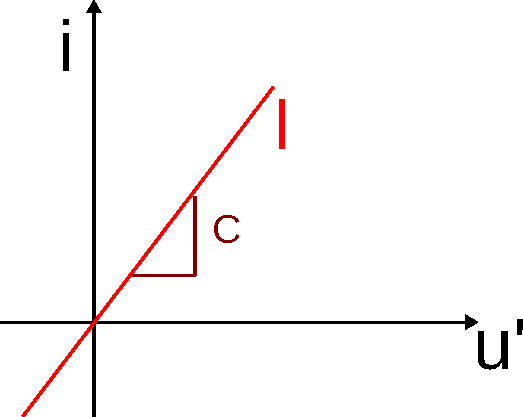
\includegraphics[scale=0.3]{c1-fig4}
\subsection{Bobine idéale}
C'est un dip\^ole dont la tension à ses bornes et le courant sont reliés par : \(U = L \frac{\mathrm{d}i}{\mathrm{d}t}\) où $L$ est l'inductance propre de la bobine (en Henry H) .

Pour un courant constant, on a une tension nulle, donc cela se comporte comme un court-circuit.

Pour la fabriquer, on réalise un enroulement de fil conducteur (souvant autour d'un barreau ferro-magnétique). \(L\) dépend ud nombre de tour, du diamètre du tube et des prorpriétés du barrea, la permeabilité lagnétique relative

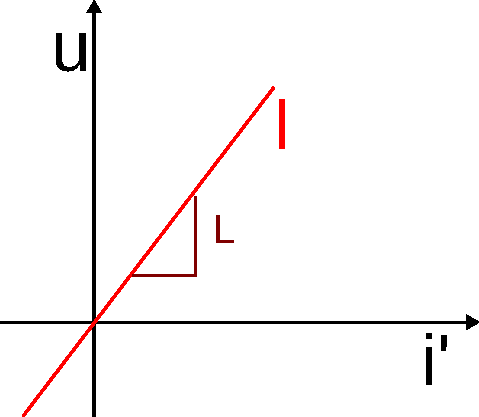
\includegraphics[scale=0.3]{c1-fig5}
\end{document}

